\begin{appendix}
\section{Molecular spectra}
%-------------------------------------------------------------------------------
\begin{figure}[ht]
  \begin{center}
    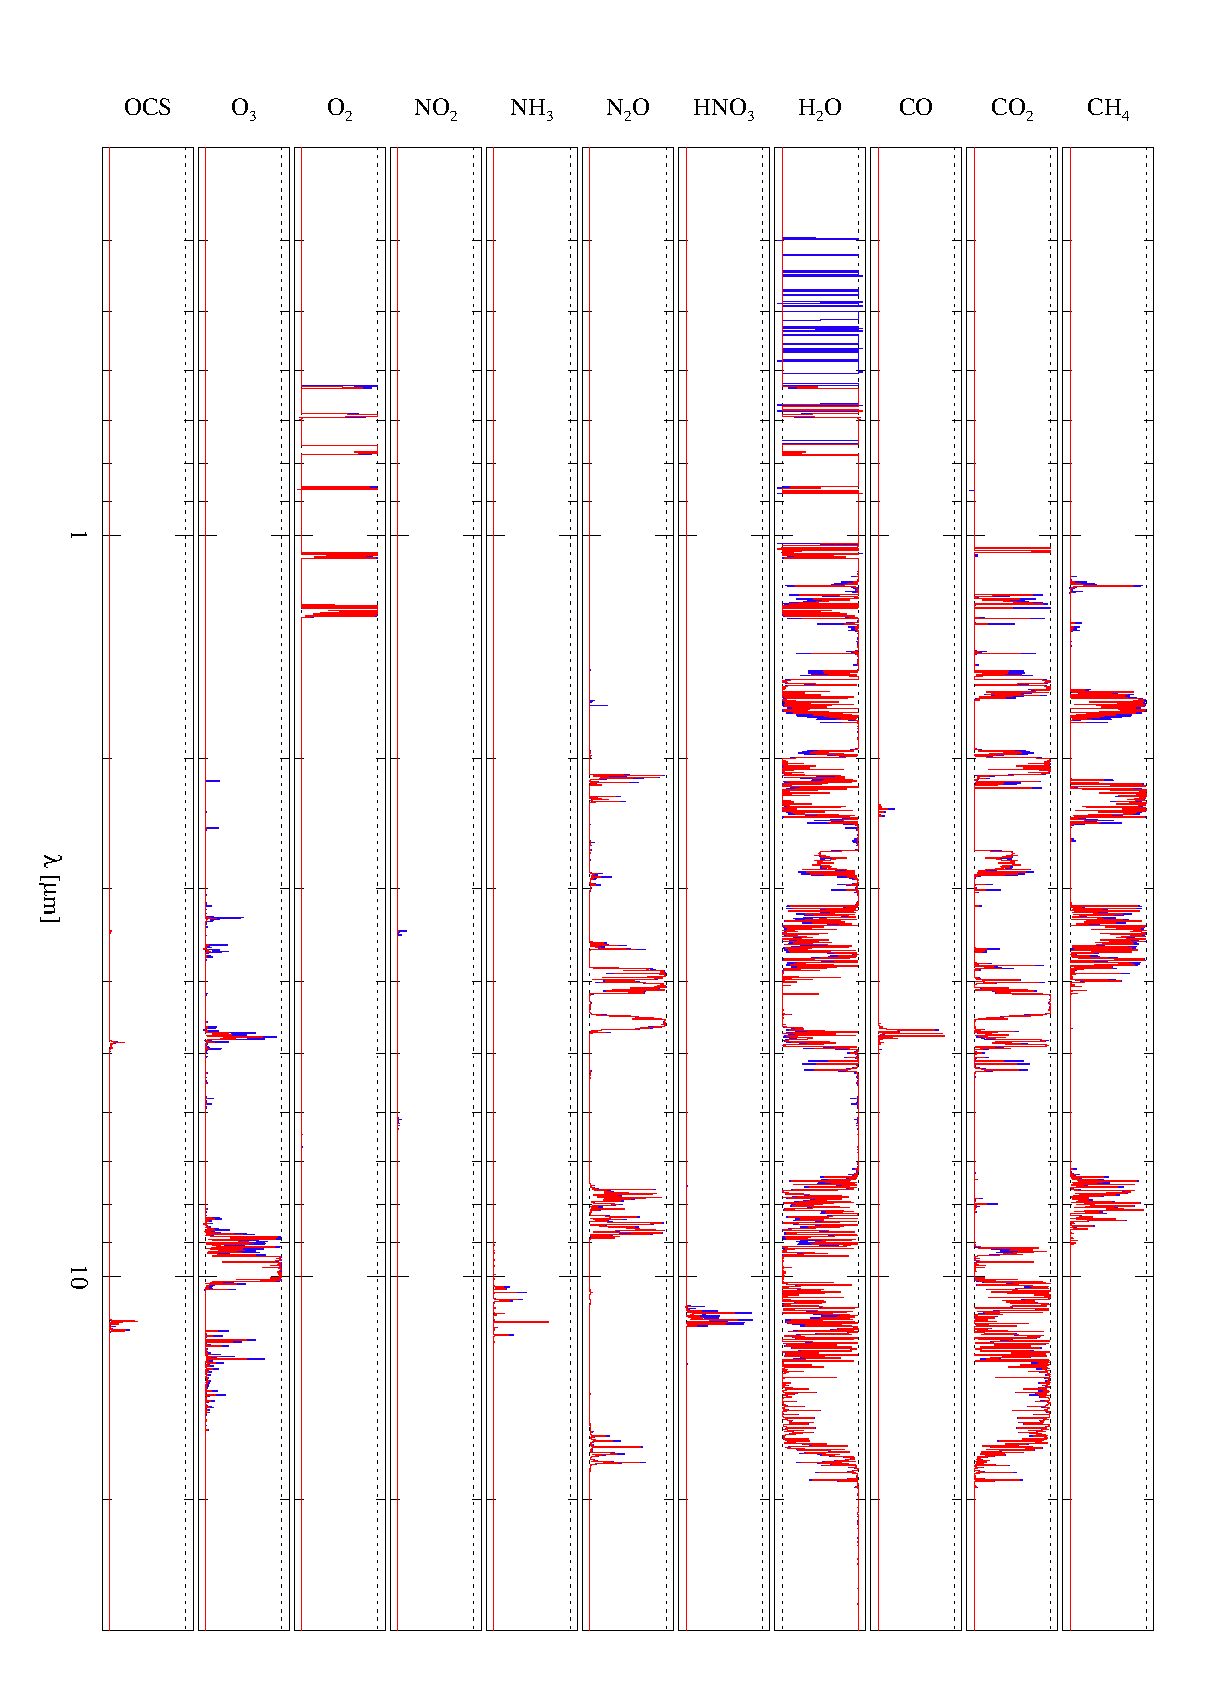
\psfig{file=figures/cheat_sheet_RT.eps,width=0.97\textwidth,angle=0}
    \caption{{\it Influence of individual molecules as a function of
    wavelength:} this figure shows the relative importance of all molecules at
    a given wavelength, which exceed more than 5\% of the total radiance (in
    red) or transmission (in blue). See text for more detail.}
    \label{fig:molecs_all}
  \end{center}
\end{figure}
%-------------------------------------------------------------------------------
\begin{figure}[ht]
  \begin{center}
    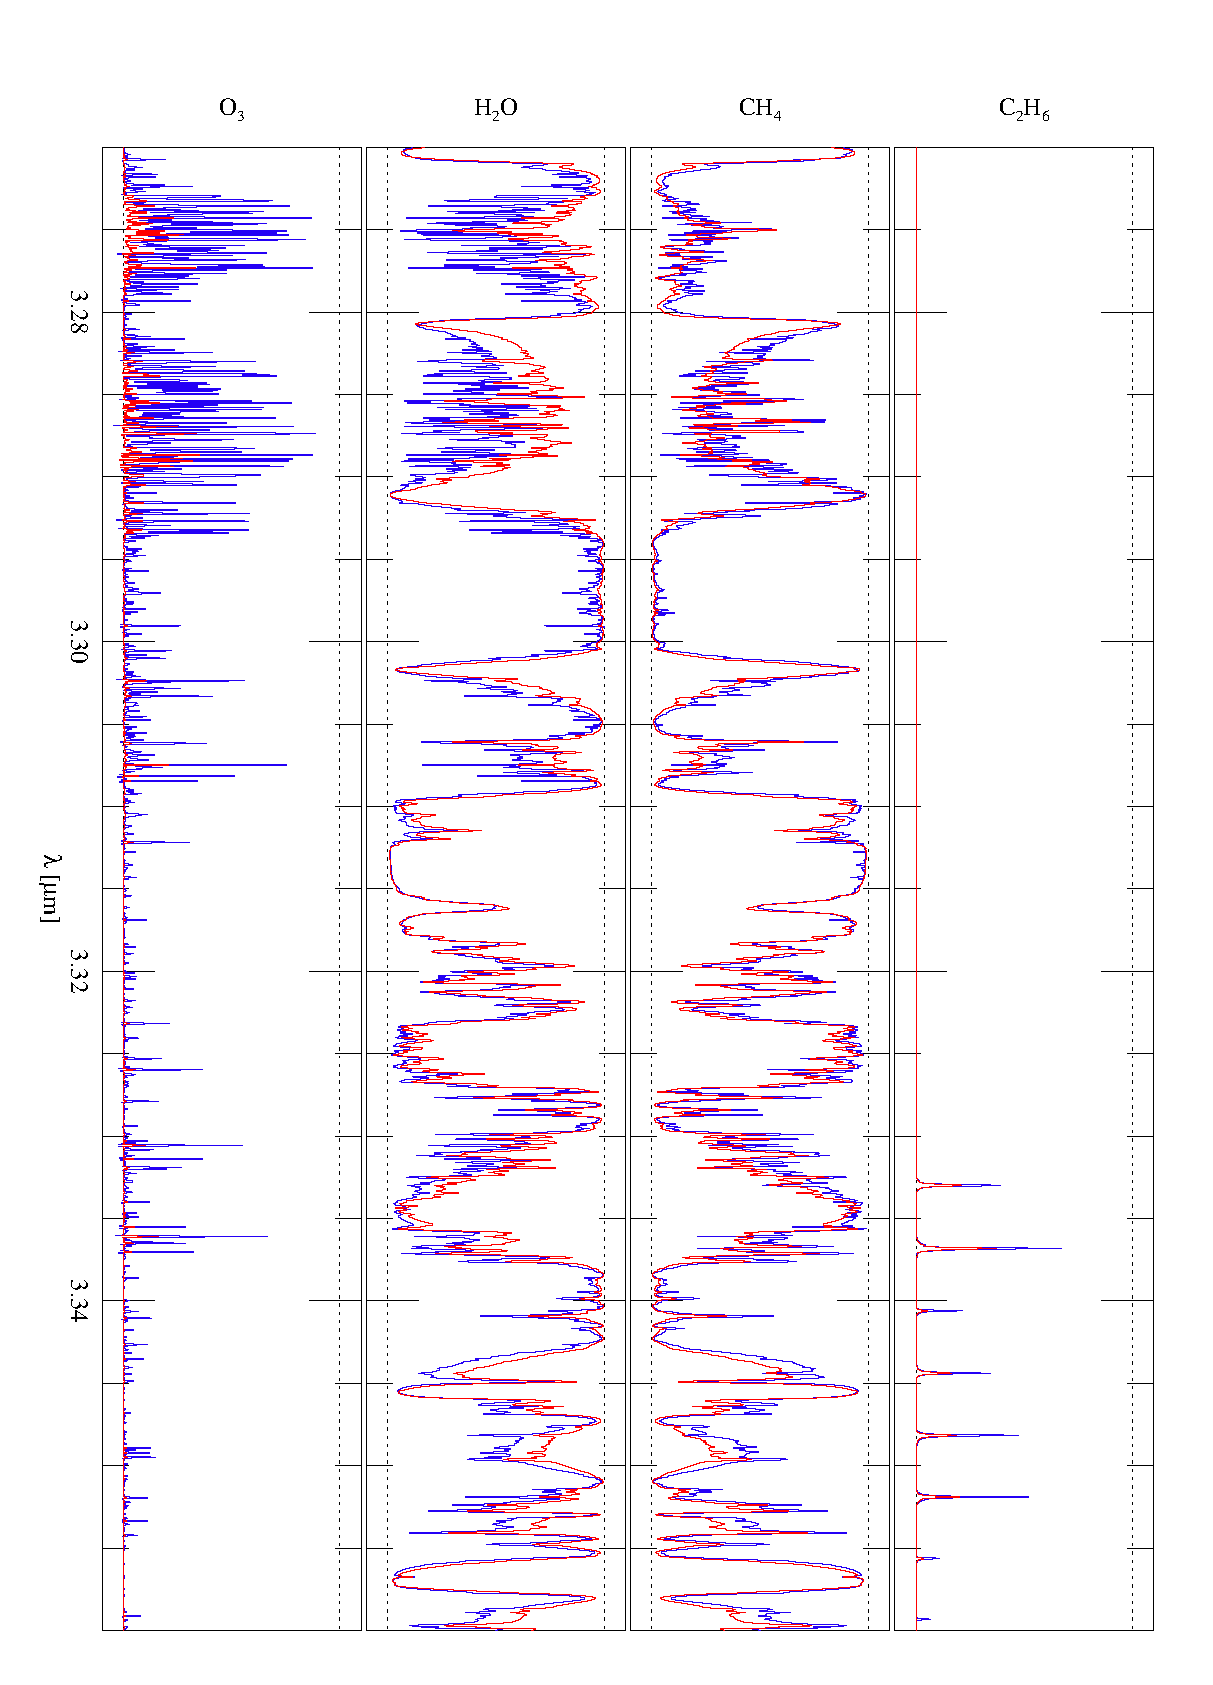
\psfig{file=figures/crires_RT.eps,width=0.97\textwidth,angle=0}
    \caption{{\it Influence of individual molecules as a function of
    wavelength:} same as Figure~\ref{fig:molecs_all}, but for the CRIRES test
    data wavelength regime. See text for more detail.}
    \label{fig:molecs_crires}
  \end{center}
\end{figure}
%-------------------------------------------------------------------------------
\begin{figure}[ht]
  \begin{center}
    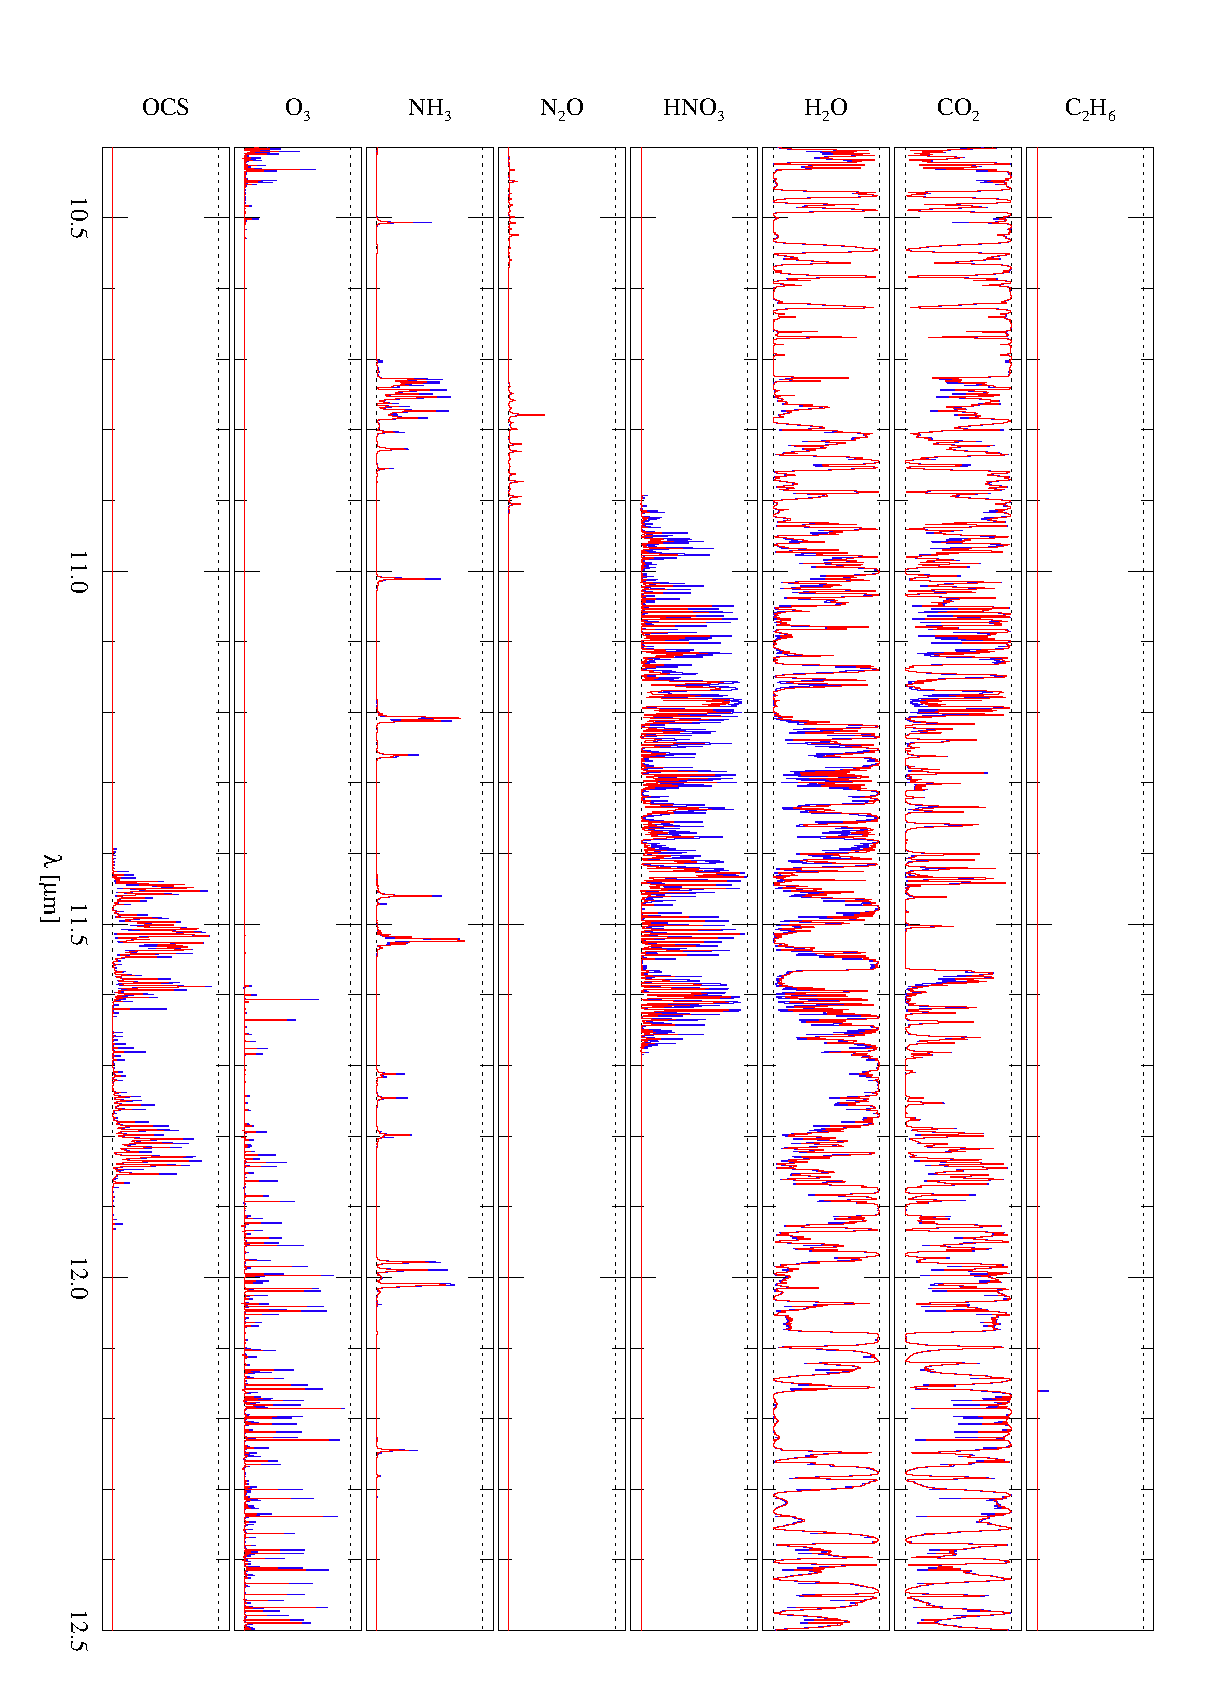
\psfig{file=figures/visir3_RT.eps,width=0.97\textwidth,angle=0}
    \caption{{\it Influence of individual molecules as a function of
    wavelength:} same as Figure~\ref{fig:molecs_all}, but for the VISIR test
    data wavelength regime. See text for more detail.}
    \label{fig:molecs_visir3}
  \end{center}
\end{figure}
%-------------------------------------------------------------------------------
\begin{figure}[ht]
    \begin{center}
    \psfig{file=figures/visir4_RT.eps,width=0.97\textwidth,angle=0}
    \caption{{\it Influence of individual molecules as a function of
    wavelength:} same as Figure~\ref{fig:molecs_all}, but for the VISIR test
    data wavelength regime. See text for more detail.}
    \label{fig:molecs_visir4}
  \end{center}
\end{figure}
%-------------------------------------------------------------------------------
\begin{figure}[ht]
  \begin{center}
    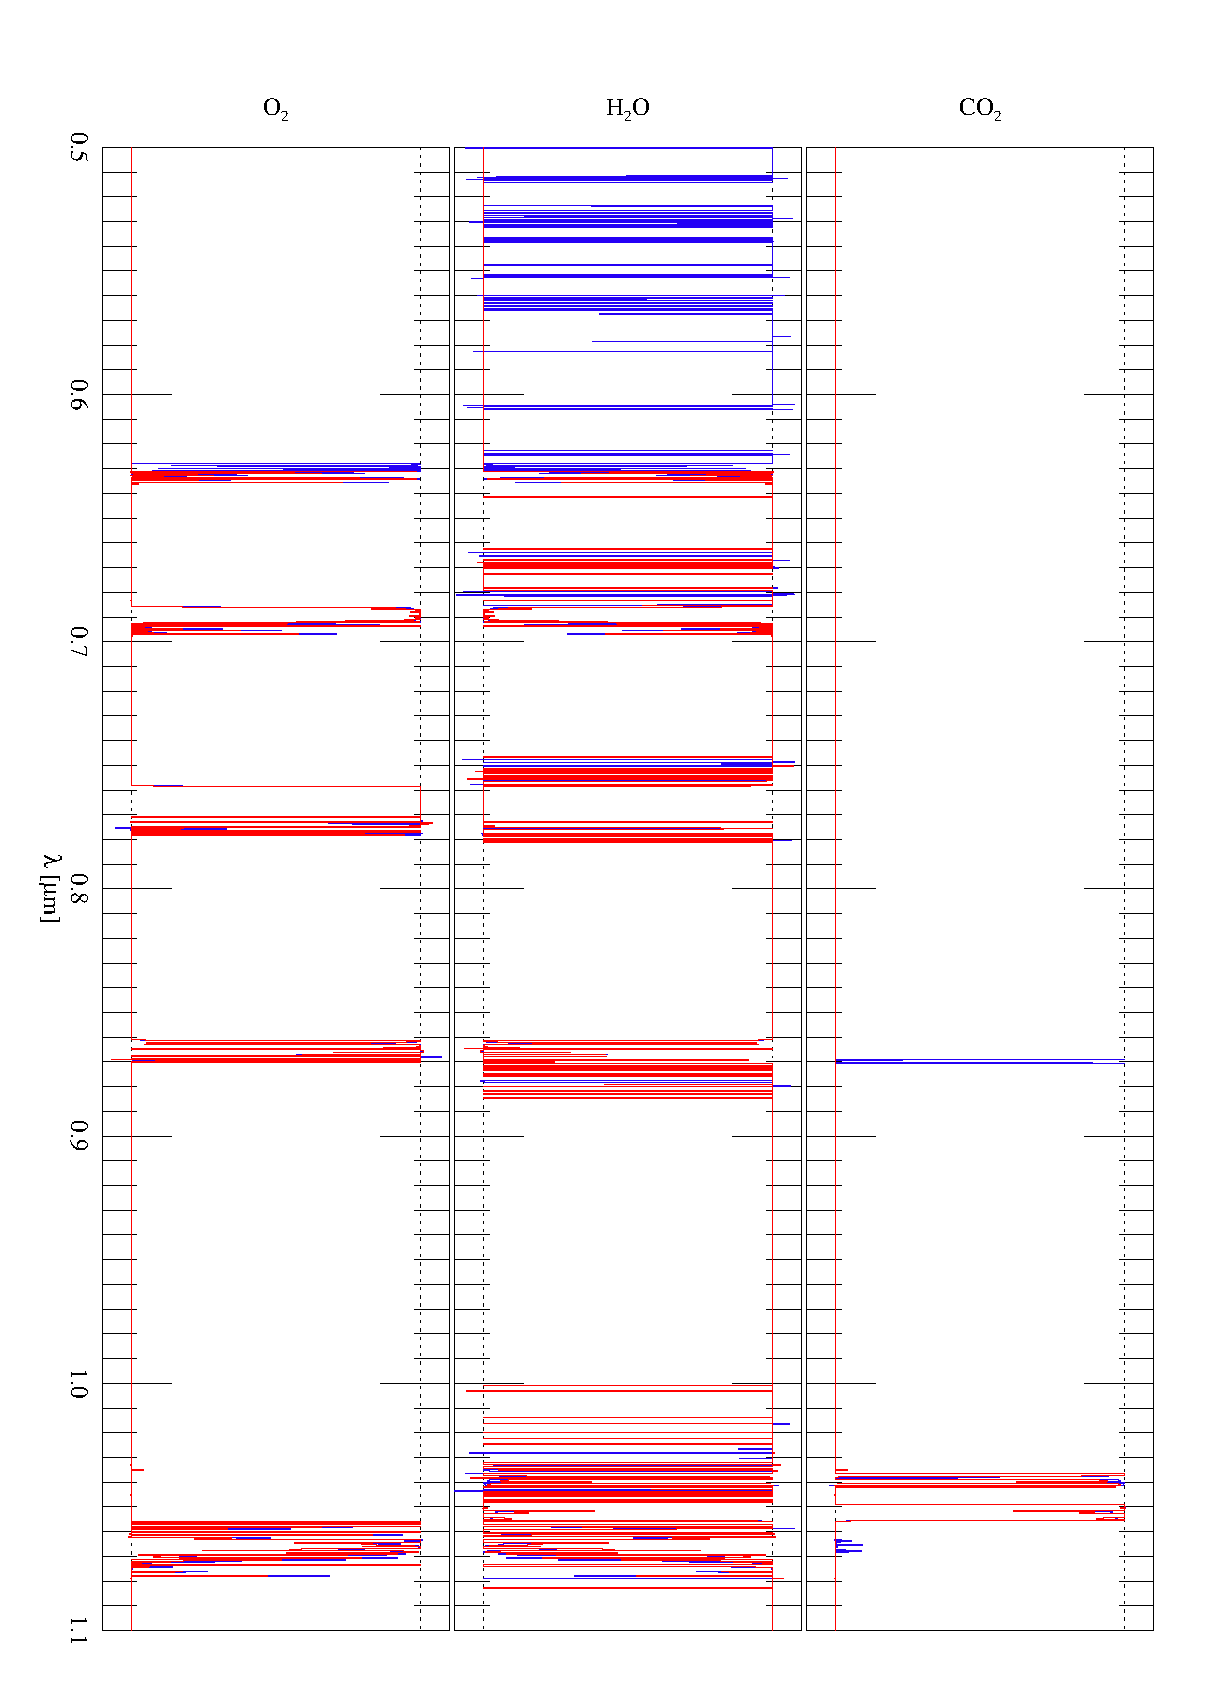
\psfig{file=figures/xshooter_RT.eps,width=0.97\textwidth,angle=0}
    \caption{{\it Influence of individual molecules as a function of
    wavelength:} same as Figure~\ref{fig:molecs_all}, but for the X-Shooter
    VIS-arm test data wavelength regime. See text for more detail.}
    \label{fig:molecs_xshoo}
  \end{center}
\end{figure}
%-------------------------------------------------------------------------------
\end{appendix}
